\documentclass{article}
\usepackage{amsthm,amsmath,amsfonts,amssymb,mathtools}
\usepackage[colorlinks,citecolor=blue,urlcolor=blue]{hyperref}
\usepackage{enumitem}
\usepackage[margin=1in]{geometry}

\usepackage{listings}

% Some useful macros.
\newcommand{\given}{\,|\,}
\newcommand{\trans}{\mathsf{T}}
\newcommand{\bx}{\mathbf{x}}
\newcommand{\by}{\mathbf{y}}
\newcommand{\bw}{\mathbf{w}}
\newcommand{\distNorm}{\mathcal{N}}
\newcommand{\bzero}{\mathbf{0}}
\newcommand{\btheta}{\boldsymbol{\theta}}
\newcommand{\bpi}{\boldsymbol{\pi}}
\newcommand{\ep}{\varepsilon}
\def\ie{i.e.\ }
\def\eg{e.g.\ }
\def\iid{i.i.d.\ }
\def\simiid{\sim_{\mbox{\tiny iid}}}
\newcommand{\varv}{\mathbb{V}}
\newcommand{\LL}[1]{\frac{\partial \log \pi(a_{#1}| s_{#1}, \theta)}{\partial \theta}}
\newcommand{\PT}{\frac{\partial}{\partial \theta}}
\newcommand{\PP}[1]{\frac{\partial}{\partial #1}}
\newcommand{\PPH}{\frac{\partial}{\partial \phi}}
\newcommand{\LP}[1]{\PT \log p(#1)}
\newcommand{\LZ}[1]{\frac{\log \pi(z_{#1}| s_{#1}, \theta)}{\partial \theta}}
\newcommand{\N}{\mathcal{N}}

\begin{document}
\title{Assignment 3: Variational Autoencoders}
\author{STA414/STA2014 and CSC412/CSC2506 Winter 2020\\
  (Bill) Yuan Liu\\
  Student Number: 996954078
}
\maketitle

\subsection{Background}
In this assignment, we will implement and investigate the Variational Autoencoder on binarized MNIST digits, as introduced by the paper \href{https://arxiv.org/pdf/1312.6114.pdf}{Auto-Encoding Variational Bayes} by Kingma and Welling (2013). Before starting, we recommend reading this paper.

\paragraph{Data.}
Each datapoint in the \href{http://yann.lecun.com/exdb/mnist/}{MNIST} dataset is a 28x28 grayscale image (i.e. pixels are values between 0 and 1) of a handwritten digit in $\{0 \dots 9\}$, and a label indicating which number.
MNIST is the `fruit fly' of machine learning -- a simple standard problem useful for comparing the properties of different algorithms.

Use the first 10000 samples for training, and the second 10000 for testing.
Hint: Also build a dataset of only 100 training samples to use when debugging, to make loading and training faster.

\paragraph{Tools.}
As before, you can (and should) use automatic differentiation provided by your package of choice.
Whereas in previous assignments you implemented neural network layers and stochastic gradient descent manually, in this assignment feel free to use those provided by a machine learning framework.
In Julia, these will be provided by \texttt{Flux.jl}.
You can also freely copy and adapt the Python autograd starter code provided.  
If you do, you should probably remove batch normalization.

However, you \textbf{may not use any probabilistic modelling elements} from these frameworks.
In particular, sampling from and evaluating densities under distributions must be written by you or provided by the starter code.


\subsection{Model Definition}

\paragraph{Prior.}
The prior over each digit's latent representation is a multivariate standard normal distribution.
For all questions, we'll set the dimension of the latent space $D_z$ to 2.
A larger latent dimension would provide a more powerful model, but for this assignment we'll use a two-dimensional latent space to make visualization and debugging easier..


\paragraph{Likelihood.}
Given the latent representation $z$ for an image, the distribution over all 784 pixels in the image is given by a product of independent Bernoullis, whose means are given by the output of a neural network $f_\theta(z)$:
$$p(x|z, \theta) = \prod_{d=1}^{784} \operatorname{Ber}(x_d|f_\theta(z)_d)$$
The neural network $f_\theta$ is called the decoder, and its parameters $\theta$ will be optimized to fit the data.


\pagebreak
\section{Implementing the Model [5 points]}

For your convenience we have provided the following functions:
\begin{itemize}
  \item \texttt{factorized\_gaussian\_log\_density} that accepts the mean and \textbf{log} standard deviations for a product of independent gaussian distribtuions and computes the likelihood under them. This function will produce the log-likelihood for each batch element $1 \times B$
  \item \texttt{bernoulli\_log\_density} that accepts the logits of a bernoulli distribution over $D$-dimensional data and returns $D \times B$ log-likelihoods.
  \item \texttt{sample\_diag\_gaaussian} that accepts above parameters for a factorized Gaussian distribution and samples with the reparameterization trick.
  \item \texttt{sample\_bernoulli} that accepts above parameters for a Bernoulli distribution and samples from it.
  \item \texttt{load\_binarized\_mnist} that loads and binarizes the MNIST dataset.
  \item \texttt{batch\_x} and \texttt{batch\_x} that splits the data, and just the images, into batches.
\end{itemize}

Further, in the file \texttt{example\_flux\_model.jl} we demonstrate how to specify neural network layers with Flux library.
Note that Flux provides convenience functions that allow us to take gradients of functions with respect to parameters that \textbf{are not passed around explicitly}.
Other AD frameworks, of if you prefer to implement your own network layers, recycling code from previous assignments, you may need to explicilty provide the network parameters to the functions below.

\begin{enumerate}[label=(\alph*)]
	% \item {\bf [2 points]} Load the MNIST dataset, and binarize the images.
	% That is, all the pixels with brightness more than 127 out of 255 should be set to 1, and all others set to 0.
	% Take the first 10000 images as a training set. %, and a separate test set of 10000 images.
	% Also, keep the image labels with the corresponding images.
	
\item {\bf [1 point]} Implement a function \texttt{log\_prior} that computes the log of the prior over a digit's representation $\log p(z)$.

\begin{lstlisting}[
  mathescape,
  columns=fullflexible,
  basicstyle=\ttfamily,breaklines=true
  ]
  log_prior(z) = factorized_gaussian_log_density(0,0,z)
\end{lstlisting}

  \item {\bf [2 points]} Implement a function \texttt{decoder} that, given a latent representation $z$ and a set of neural network parameters $\theta$ (again, implicitly in Flux), produces a 784-dimensional mean vector of a product of Bernoulli distributions, one for each pixel in a $28 \times 28$ image.
	Make the decoder architecture a multi-layer perceptron (i.e. a fully-connected neural network) with a single hidden layer with $500$ hidden units, and a \texttt{tanh} nonlinearity.
  Its input will be a batch two-dimensional latent vectors ($z$s in $D_z \times B$) and its output will be a 784-dimensional vector representing the logits of the Bernoulli means for each dimension $D_\text{data}\times B$.
	For numerical stability, instead of outputting the mean $\mu \in [0,1]$, you should output $\log \left( \frac{\mu}{1 - \mu} \right) \in \mathbb{R}$ called ``logit".

\begin{lstlisting}[
  mathescape,
  columns=fullflexible,
  basicstyle=\ttfamily,breaklines=true
  ]
  Dz, Dh = 2, 500
  Ddata = 28^2
  
  decoder = Chain(Dense(Dz, Dh, tanh), Dense(Dh, Ddata))
\end{lstlisting}

	% \item {\bf [3 points]} Implement a function \texttt{log\_prod\_Bernoulli} that, given an array of transformed Bernoulli mean parameters $\log \left( \frac{\mu}{1 - \mu} \right)$ and an equally-sized binary array $x$, computes the log-likelihood $\log \prod_d \operatorname{Ber}(x|\mu)$.
	% Hint: for numerical stability, you should use something like logaddexp to compute the Bernoulli log-probabilities.
	% It's easy to make a mistake here, so you might want to write a test for this function.
	
	\item {\bf [1 point]} Implement a function \texttt{log\_likelihood} that, given a latent representation $z$ and a binarized digit $x$, computes the log-likelihood $\log p(x|z)$.
\begin{lstlisting}[
  mathescape,
  columns=fullflexible,
  basicstyle=\ttfamily,breaklines=true
  ]
  function log_likelihood(x,z)
  logit_mean = decoder(z)
  return sum(bernoulli_log_density(logit_mean,x),dims=1)
  end
\end{lstlisting}
        
   \item {\bf [1 point]} Implement a function \texttt{joint\_log\_density} which combines the log-prior and log-likelihood of the observations to give $\log p(z, x)$ for a single image.

\begin{lstlisting}[
  mathescape,
  columns=fullflexible,
  basicstyle=\ttfamily,breaklines=true
  ]
  joint_log_density(x,z) = log_prior(z) .+ log_likelihood(x,z)
\end{lstlisting}

\end{enumerate}

\pagebreak
\section{Amortized Approximate Inference and training [13 points]}
\begin{enumerate}[label=(\alph*)]
  \item {\bf [2 points]} Write a function \texttt{encoder} that, given an image $x$ (or batch of images) and recognition parameters $\phi$, evaluates an MLP to outputs the mean and log-standard deviation of a factorized Gaussian of dimension $D_z = 2$.
	Make the encoder architecture a multi-layer perceptron (i.e. a fully-connected neural network) with a single hidden layer with $500$ hidden units, and a \texttt{tanh} nonlinearity.
	This function must be able to be evaluated in parallel on a batch of images, using the same parameters $\phi$ for each image.

\begin{lstlisting}[
  mathescape,
  columns=fullflexible,
  basicstyle=\ttfamily,breaklines=true
  ]
encoder = Chain(Dense(Ddata, Dh, tanh),
                  Dense(Dh, Dz*2),
                  unpack_gaussian_params)
\end{lstlisting}
        
  \item {\bf [1 points]} Write a function \texttt{log\_q} that given the parameters of the variational distribution, evaluates the likelihood of $z$.

\begin{lstlisting}[
  mathescape,
  columns=fullflexible,
  basicstyle=\ttfamily,breaklines=true
  ]
  log_q(q_$\mu$,q_log$\sigma$, z) =  factorized_gaussian_log_density(q_$\mu$, q_log$\sigma$, z)
\end{lstlisting}
                
\item {\bf [5 points]} Implement a function \texttt{elbo} which computes an unbiased estimate of the mean variational evidence lower bound on a batch of images.
	Use the output of \texttt{encoder} to give the parameters for $q_\phi(z|\text{data})$.
	This estimator takes the following arguments:
	\begin{itemize}
		\item \texttt{x}, an batch of $B$ images, $D_x \times B$.
    \item \texttt{encoder\_params}, the parameters $\phi$ of the encoder (recognition network). Note: these are not required with Flux as parameters are implicit.
		\item \texttt{decoder\_params}, the parameters $\theta$ of the decoder (likelihood). Note: these are not required with Flux as parameters are implicit.
	\end{itemize}
	This function should return a single scalar.
	Hint: You will need to use the reparamterization trick when sampling \texttt{zs}.
	You can use any form of the ELBO estimator you prefer.
  (i.e., if you want you can write the KL divergence between q and the prior in closed form since they are both Gaussians).
	You only need to sample a single $z$ for each image in the batch.

\begin{lstlisting}[
  mathescape,
  columns=fullflexible,
  basicstyle=\ttfamily,breaklines=true
  ]
function elbo(x)
    (q_$\mu$, q_log$\sigma$) = encoder(x)
    z = sample_diag_gaussian(q_$\mu$, q_log$\sigma$)
    likelihoods = log_likelihood(x,z)
    negative_kl = 1/2 * sum(1 .+ 2 .* q_log$\sigma$ .-
                               q_$\mu$ .* q_$\mu$ .-
                               exp.(2 .* q_log$\sigma$), dims=1)
    mean(negative_kl + likelihoods, dims=2)[1]
end
\end{lstlisting}
  
	\item {\bf [2 points]} Write a loss function called \texttt{loss}
          that returns the negative elbo estimate over a batch of data.

\begin{lstlisting}[
  mathescape,
  columns=fullflexible,
  basicstyle=\ttfamily,breaklines=true
  ]
function loss(x)
    return -elbo(x)
end
\end{lstlisting}
\pagebreak
\item {\bf [3 points]} Write a function that initializes and optimizes the encoder and decoder parameters jointly on the training set. 
    Note that this function should optimize with gradients on the elbo estimate over batches of data, not the entire dataset.
    Train the data for 100 epochs (each epoch involves a loop over every batch).
    Report the final ELBO on the test set.
    Tip: Save your trained weights here (e.g.\ with \texttt{BSON.jl}, see starter code, or by pickling in Python) so that you don't need to train them again.

\begin{lstlisting}[
  mathescape,
  columns=fullflexible,
  basicstyle=\ttfamily,breaklines=true
  ]
function train_model_params!(loss, encoder, decoder, train_x, test_x; nepochs=10)
  ps = Flux.params(encoder, decoder)
  opt = ADAM(0.0025)
  for i in 1:nepochs
    for d in batch_x(train_x,1000)
      gs  = Flux.gradient(()->loss(d), ps)
      Flux.Optimise.update!(opt,ps,gs)
    end
    if i%1 == 0 # change 1 to higher number to compute and print less frequently
      @info "Test loss at epoch $i: $(loss(batch_x(test_x)[1]))"
    end
  end
  @info "Parameters of encoder and decoder trained!"
end


## Train the model
train_model_params!(loss,encoder,decoder,train_x,test_x, nepochs=100)
\end{lstlisting}

Trained on 10000 samples. Final test loss on last epoch: 161.

\end{enumerate}

\pagebreak

\section{Visualizing Posteriors and Exploring the Model [15 points]}
In this section we will investigate our model by visualizing the distribution over data given by the generative model, sampling from it, and interpolating between digits.

\begin{enumerate}[label=(\alph*)]
	\item {\bf [5 points]} Plot samples from the trained generative model using ancestral sampling:	
	\begin{enumerate}[label=(\alph*)]

			\item First sample a z from the prior.
			\item Use the generative model to compute the bernoulli means over the pixels of $x$ given $z$. Plot these means as a greyscale image.
			\item Sample a binary image $x$ from this product of Bernoullis. Plot this sample as an image.
	\end{enumerate}
	Do this for 10 samples z from the prior.
	
	Concatenate all your plots into one 2x10 figure where each image in the first row shows the Bernoulli means of $p(x|z)$ for a separate sample of $z$, and each image in the the second row is a bianry image, sampled from the distribution above it.
	Make each column an independent sample.

\begin{lstlisting}[
  mathescape,
  columns=fullflexible,
  basicstyle=\ttfamily,breaklines=true
  ]
number_of_samples = 10

sample_z = randn((2,number_of_samples))
logit_mean = decoder(sample_z)
bernoulli_mean = 1.0 ./ (1.0 .+ exp.(-logit_mean))
sample_images = sample_bernoulli(bernoulli_mean)

plots_ber = []
plots_bin = []
for i in 1:number_of_samples
     push!(plots_ber, plot(mnist_img(bernoulli_mean[:,i])))
     push!(plots_bin, plot(mnist_img(sample_images[:,i])))
end

plots = [ plots_ber; plots_bin ]
rows = Int(number_of_samples*2/10)
display(plot(plots...,
              layout=grid(rows,10),
              size =(150*10, 150*rows),
              axis=nothing))

savefig(joinpath("plots","3a.png"))
\end{lstlisting}

\begin{figure}[h]
  \centering
  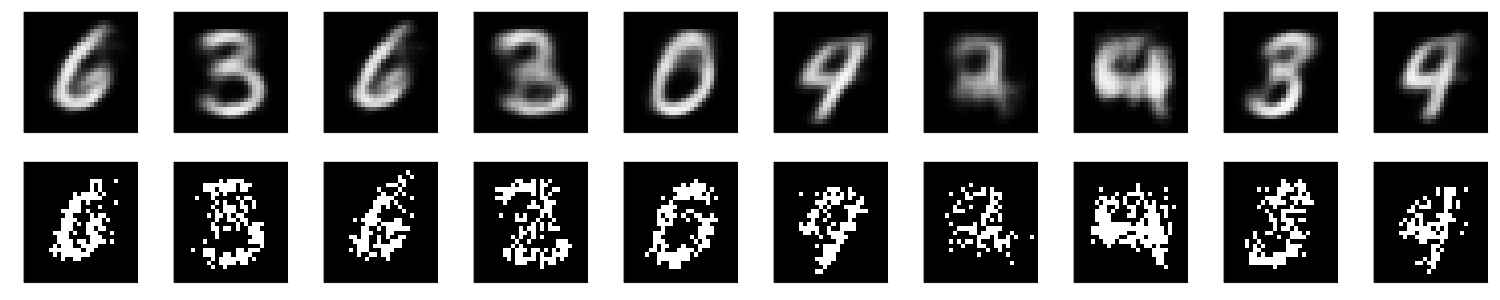
\includegraphics[width=16cm]{plots/3a.png}
  \caption{Generative Samples $p(x|z)$. Top: mean. Bottom: binarized}
\end{figure}

\pagebreak
     
	\item {\bf [5 points]} One way to understand the meaning of latent representations is to see which parts of the latent space correspond to which kinds of data.
	Here we'll produce a scatter plot in the latent space, where each point in the plot represents a different image in the training set.
	%will be the mean vector for the distribution $q_\phi(z|x)$ given by the encoder. Further, we will colour each point in the plot by the class label for the input data.
	
	\begin{enumerate}[label=(\alph*)]
		\item Encode each image in the training set.
		\item Take the 2D mean vector of each encoding $q_\phi(z|x)$.
		\item Plot these mean vectors in the 2D latent space with a scatterplot.
		\item Colour each point according to the class label (0 to 9).
	\end{enumerate}
	
	Hopefully our latent space will group images of different classes, even though we never provided class labels to the model!

\begin{lstlisting}[
  mathescape,
  columns=fullflexible,
  basicstyle=\ttfamily,breaklines=true
  ]
mean_vector_x = [[] for i = 1:10]
mean_vector_y = [[] for i = 1:10]
mean_label = ["0" "1" "2" "3" "4" "5" "6" "7" "8" "9"]
for i in 1:size(train_x)[2]
  (mu, logsig) = encoder(train_x[:,i])
  push!(mean_vector_x[train_label[i]+1], mu[1])
  push!(mean_vector_y[train_label[i]+1], mu[2])
end
plot(mean_vector_x,
     mean_vector_y,
     seriestype = :scatter,
     xlabel="z1 mean",
     ylabel="z2 mean",
     label=mean_label)
savefig(joinpath("plots","3b.png"))
\end{lstlisting}
\begin{figure}[h]
  \centering
  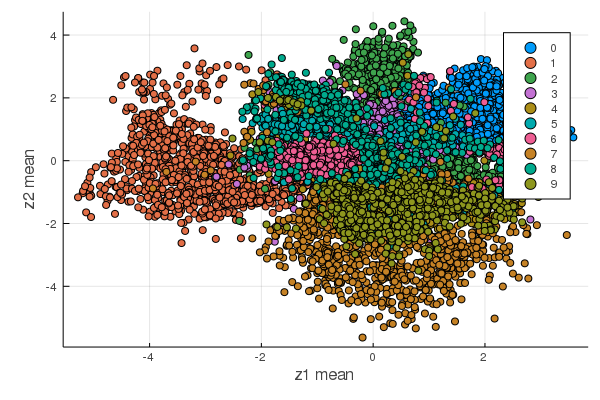
\includegraphics[width=14cm]{plots/3b.png}
  \caption{Latent Space Encoding on Training Set Sample}
\end{figure}

	\item {\bf [5 points]} Another way to examine a latent variable model with continuous latent variables is to interpolate between the latent representations of two points.
	
	Here we will encode 3 pairs of data points with different classes. Then we will linearly interpolate between the mean vectors of their encodings. We will plot the generative distributions along the linear interpolation.
	
	\begin{enumerate}[label=(\alph*)]
		\item First, write a function which takes two points $z_a$ and $z_b$, and a value $\alpha \in [0,1]$, and outputs the linear interpolation $z_\alpha = \alpha z_a + (1 - \alpha) z_b$.
		\item Sample 3 pairs of images, each having a different class.
		\item Encode the data in each pair, and take the mean vectors
		\item Linearly interpolate between these mean vectors
		\item At 10 equally-space points along the interpolation, plot the Bernoulli means $p(x|z_\alpha)$
		\item Concatenate these plots into one figure.
        \end{enumerate}

\begin{lstlisting}[
  mathescape,
  columns=fullflexible,
  basicstyle=\ttfamily,breaklines=true
]
function interp(a, b, alpha)
  alpha .* a + (1-alpha) .* b
end
image_samples = [ (train_x[:,3889],train_x[:,9000]), #,0 9
                  (train_x[:,499],train_x[:,600]), # 6, 7
                  (train_x[:,9137],train_x[:,99]), #1, 3
                ]
image_samples_encode = map(x -> (encoder(x[1]), encoder(x[2])), image_samples)
plots_interp = []
for i in 1:3
  (enc_a, enc_b) = image_samples_encode[i]
  mu_a = enc_a[1]
  mu_b = enc_b[1]
  sig_a = exp.(enc_a[2])
  sig_b = exp.(enc_b[2])
  for j in 0:10
    alpha = j/10.0
    mu_alpha = interp(mu_a, mu_b, alpha)
    sig_alpha = interp(sig_a, sig_b, alpha)
    logit_mean = decoder(mu_alpha)
    reconstruct = exp.(logit_mean) ./ (1 .+ exp.(logit_mean))
    push!(plots_interp, plot(mnist_img(reconstruct[:])))
  end
end
display(plot(plots_interp..., layout=grid(3,11), size =(1000, 200), axis=nothing))
savefig(joinpath("plots","3c.png"))
\end{lstlisting}
\begin{figure}[h]
  \centering
  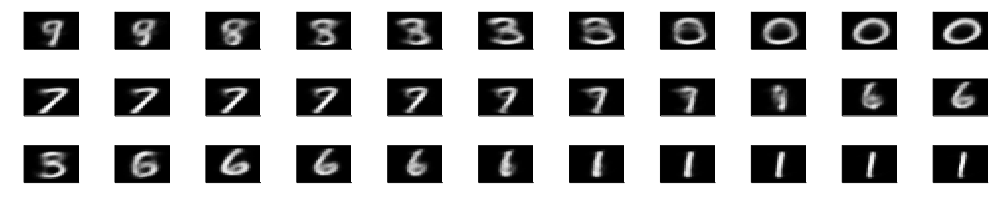
\includegraphics[width=17cm]{plots/3c.png}
  \caption{Generative Ouput from Latent Space Interpolation over Pairs of Samples}
\end{figure}

\end{enumerate}


\pagebreak

\section{Predicting the Bottom of Images given the Top [15 points]}

Now we'll use the trained generative model to perform inference for $p(z|\text{top half of image x})$.
Unfortunately, we can't re-use our recognition network, since it can only input entire images.
However, we can still do approximate inference without the encoder.

To illustrate this, we'll approximately infer the distribution over the pixels in the bottom half an image conditioned on the top half of the image:
$$p(\text{bottom half of image x} | \text{top half of image x}) = \int p(\text{bottom half of image x} | z) p( z | \text{top half of image x}) dz$$
To approximate the posterior $p( z | \text{top half of image x})$, we'll use stochastic variational inference.

\begin{enumerate}[label=(\alph*)]	
	\item {\bf [5 points]} Write a function that computes $p(z, \text{top half of image x})$
	
	\begin{enumerate}[label=(\alph*)]
		\item First, write a function which returns only the top half of a 28x28 array. This will be useful for plotting, as well as selecting the correct Bernoulli parameters.
    \item Write a function that computes $\log p(\text{top half of image x} | z)$. Hint: Given $z$, the likelihood factorizes, and all the unobserved dimensions of $x$ are leaf nodes, so can be integrated out exactly. 
		\item Combine this likelihood with the prior to get a function that takes an x and an array of $z$s, and computes the log joint density $\log p(z, \text{top half of image x})$ for each $z$ in the array.
	\end{enumerate}

        \begin{lstlisting}[
  mathescape,
  columns=fullflexible,
  basicstyle=\ttfamily,breaklines=true
]
function image_top(x)
  #assume x is flattened per image
  xx = reshape(x,28,28,:)
  xxx = permutedims(xx,[2,1,3])
  xxx[1:14,1:28,:]
end
\end{lstlisting}
\begin{lstlisting}[
  mathescape,
  columns=fullflexible,
  basicstyle=\ttfamily,breaklines=true
]
function log_likelihood_image_top(x,z)
  #assume x is the top portion of the original image
  logit_mean = decoder(z)
  logit_mean_cropped = reshape(image_top_single(logit_mean), 14*28,:)
  @assert size(x)==size(logit_mean_cropped)
  sum(bernoulli_log_density(logit_mean_cropped, x), dims=1)
end
\end{lstlisting}
\begin{lstlisting}[
  mathescape,
  columns=fullflexible,
  basicstyle=\ttfamily,breaklines=true
]
function log_joint_top(x,z)
  log_prior(z) .+ log_likelihood_image_top(x,z)
end
\end{lstlisting}

	%\item {\bf [5 points]} Test your function by comparing the isocontours of $p(z | \text{top half of $x$})$ against the isocontours of $p(z | x)$.  Remember that these conditionals have the same isocontours as the joint distributions $p(z, \text{top half of $x$})$ and $p(z, x)$.  The 
	
	\item {\bf [5 points]} Now, to approximate $p(z | \text{top half of image x})$ in a scalable way, we'll use stochastic variational inference.  
    For a digit of your choosing from the training set (choose one that is modelled well, i.e. the resulting plot looks reasonable):

	\begin{enumerate}[label=(\alph*)]
		\item Initialize variational parameters $\phi_\mu$ and $\phi_{\log \sigma}$ for a variational distribution $q(z|\text{top half of $x$})$.
		\item Write a function that computes estimates the ELBO over $K$ samples $z \sim q(z|\text{top half of $x$})$.
		Use $\log p(z)$, $\log p(\text{top half of $x$} | z)$, and $\log q(z|\text{top half of $x$})$.
		\item Optimize $\phi_\mu$ and $\phi_{\log \sigma}$ to maximize the ELBO.
		\item On a single plot, show the isocontours of the joint distribution $p(z, \text{top half of image x})$, and the optimized approximate posterior $q_\phi(z | \text{top half of image x})$.
		\item Finally, take a sample $z$ from your approximate posterior, and feed it to the decoder to find the Bernoulli means of $p( \text{bottom half of image x}|z)$.  Contatenate this greyscale image to the true top of the image.
		Plot the original whole image beside it for comparison.
	\end{enumerate}

\begin{lstlisting}[
  mathescape,
  columns=fullflexible,
  basicstyle=\ttfamily,breaklines=true
]
function image_top_single(x)
  @assert size(x)[2]==1
  #assume x is flattened per image
  xx = reshape(x,28,28)
  xxx = permutedims(xx,[2,1])
  xxx[1:14,1:28]
end

function image_bottom(x)
  #assume x is flattened per image
  xx = reshape(x,28,28,:)
  xxx = permutedims(xx,[2,1,3])
  xxx[15:28,1:28,:]
end

encoder_2_in_dim = Int(Ddata/2)
encoder_2 = Chain(
  Dense(encoder_2_in_dim, Dh, tanh),
  Dense(Dh, Dz*2),
  unpack_gaussian_params)

function elbo_2(x, K=10)

  temp = image_top(x)
  xx = reshape(temp, 14*28,:)
  @assert size(xx)[1] == encoder_2_in_dim

  (z_mean, z_log_sig) = encoder_2(xx)
  samples = size(z_mean)[2]
  samples_elbo = []

  avg = 0.0

  for i in range(1,samples;step=1)
    accum = 0
    for h in range(1,K,;step=1)
      a = z_mean[:,i:i]
      b = z_log_sig[:,i:i]
      @assert size(a)==(2,1)
      @assert size(b)==(2,1)
      z_sample = sample_diag_gaussian(a, b)
      @assert size(z_sample)==(2,1)
      xxx = xx[:,i:i]
      joint = log_joint_top(xxx, z_sample)
      posterior = log_q(a, b, z_sample)
      accum += joint[1] - posterior[1]
    end
    avg += accum / samples
  end
  avg
end
function loss_2(x)
  return -elbo_2(x)
end
\end{lstlisting}
\pagebreak
\begin{lstlisting}[
  mathescape,
  columns=fullflexible,
  basicstyle=\ttfamily,breaklines=true
]  
function train_model_params_2!(loss, enc, dec, trainx, testx; nepochs=10)
  # parameters to update with gradient descent
  ps = Flux.params(enc)
  # ADAM optimizer with default parameters
  opt = ADAM(0.0025)
  # over batches of the data
  for i in 1:nepochs
    for d in batch_x(trainx,1000)
      # compute gradients with respect to variational loss over batch
      gs  = Flux.gradient(()->loss(d), ps)
      # update the paramters with gradients
      Flux.Optimise.update!(opt,ps,gs)
    end
    if i%1 == 0 # change 1 to higher number to compute and print less frequently
      @info "Test loss at epoch $i: $(loss(batch_x(testx)[1]))"
    end
  end
  @info "Parameters of encoder and decoder trained!"
end

function crop_top(xs)
  yyy = image_top(xs)
  empty = zeros(14,28,size(yyy)[3])
  tt = vcat(yyy,empty)
  ss = permutedims(reshape(tt,28,28,:),[2,1,3])
  reshape(ss,28*28,:)
end
  
idx_train = train_label .== 5
digits_train = train_x[:,idx_train]
idx_test = test_label .== 5
digits_test = test_x[:,idx_test]

train_model_params_2!(loss_2,encoder_2,decoder,digits_train, digits_test, nepochs=100)

digits_cropped_train = crop_top(digits_train)

temp = image_top(digits_cropped_train)
xx = reshape(temp, 14*28,:)
temp = encoder_2(xx)
logit_mean = decoder(temp[1])
reconstruct = 1.0 ./(1.0 .+ exp.(-logit_mean))
stitched = vcat(image_top(digits_cropped_train), image_bottom(reconstruct))
ss = reshape(permutedims(reshape(stitched,28,28,:),[2,1,3]),28*28,:)

idxs = shuffle(1:size(ss)[2])
samples = ss[:,idxs][:,1:50]

samples_original = digits_train[:,idxs][:,1:50]

plot_recon_stitch = []
plot_sample_original = []

for i in range(1,size(samples)[2],step=1)
  push!(plot_recon_stitch, plot(Gray.(reshape(samples[:,i],28,28))'))
  push!(plot_sample_original, plot(Gray.(reshape(samples_original[:,i],28,28))'))
end

display(plot(plot_sample_original..., layout=grid(5,10), size =(1500, 750), axis=nothing))
savefig(joinpath("plots","4b_e_1.png"))
display(plot(plot_recon_stitch..., layout=grid(5,10), size =(1500, 750), axis=nothing))
savefig(joinpath("plots","4b_e_2.png"))
\end{lstlisting}

\begin{figure}[h]
  \centering
  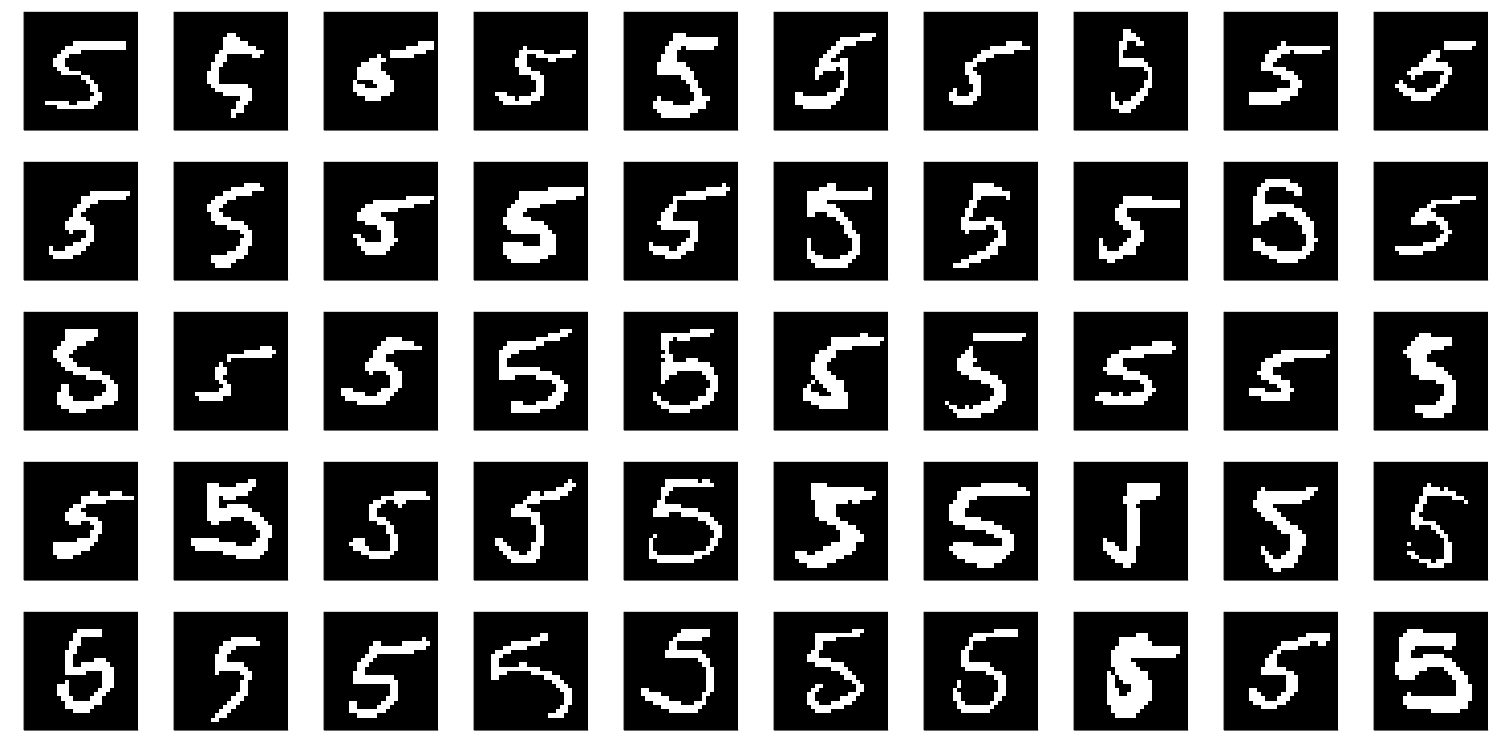
\includegraphics[width=15cm]{plots/4b_e_1.png}
  \caption{Original Samples}
\end{figure}
\begin{figure}[h]
  \centering
  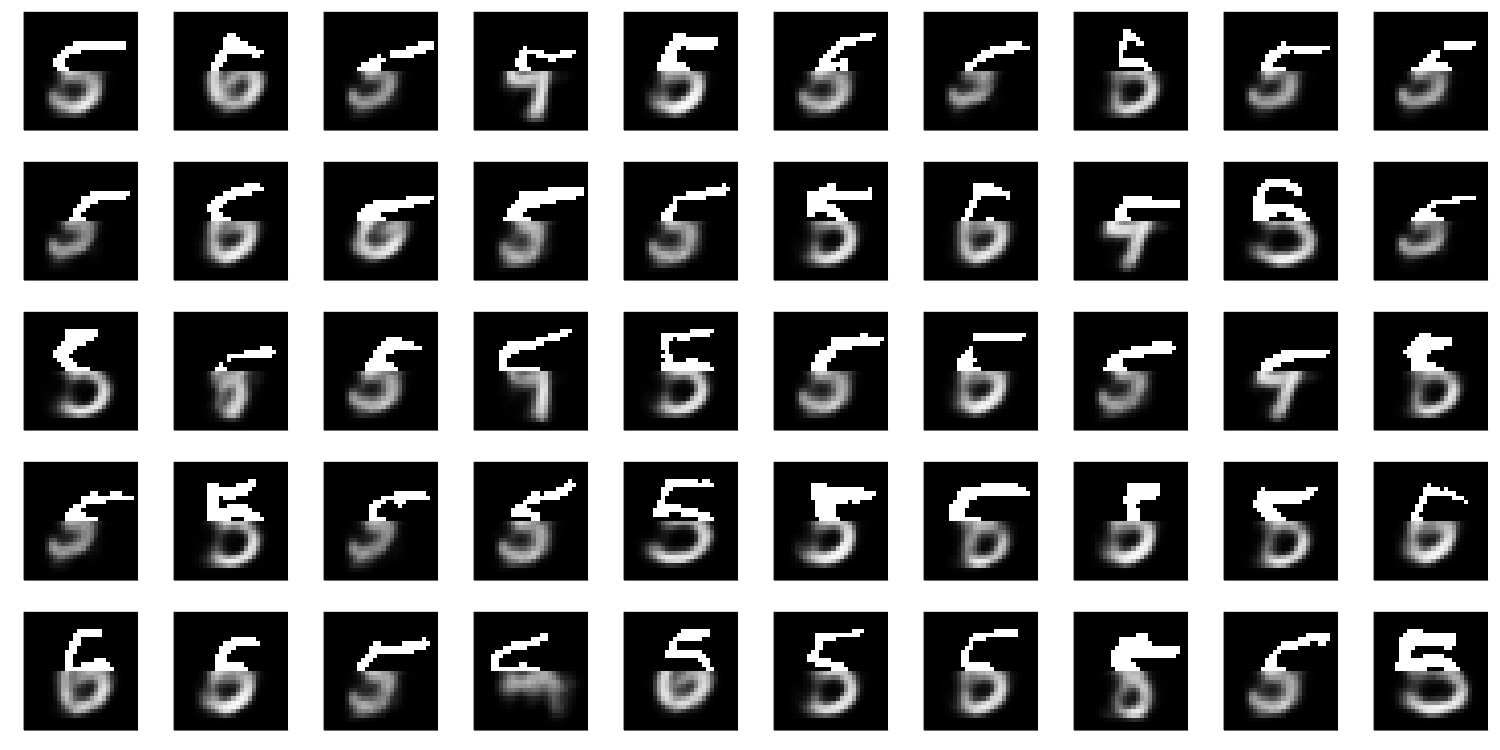
\includegraphics[width=15cm]{plots/4b_e_2.png}
  \caption{Stitched True Top and Generative Bottom}
\end{figure}

\pagebreak

\begin{lstlisting}[
  mathescape,
  columns=fullflexible,
  basicstyle=\ttfamily,breaklines=true
]
# contour plot
# select a sample
x = reshape(image_top(digits_cropped_train), 14*28,:)[:,31:31]
plot(Gray.(reshape(x,14,28)))
savefig(joinpath("plots","4b_d_sample.png"))

z1 = -4:0.07:4.0
z2 = -4:0.07:4.0

f(z1,z2) = begin
  z = zeros(2,1)
  z[1,1] = z1
  z[2,1] = z2
  v = log_joint_top(x,z)
  @assert size(v)==(1,1)
  v[1]
end

p1 = contour(z1, z2, f,
             fill=true,
             title="p(z,top half of x)")

(z_mean, z_log_sig) = encoder_2(x)

a = z_mean[:,1:1]
b = z_log_sig[:,1:1]

f2(z1,z2) = begin
  z = zeros(2,1)
  z[1,1] = z1
  z[2,1] = z2
  v = log_q(a, b, z)
  @assert size(v)==(1,1)
  v[1]
end

p2 = contour(z1, z2, f2,
             fill=true,
             title="approximate posterior q(z| top half of x)")

plot(p1,p2, size=(1000,500))
savefig(joinpath("plots","4b_d.png"))
\end{lstlisting}
\begin{figure}[h]
  \centering
  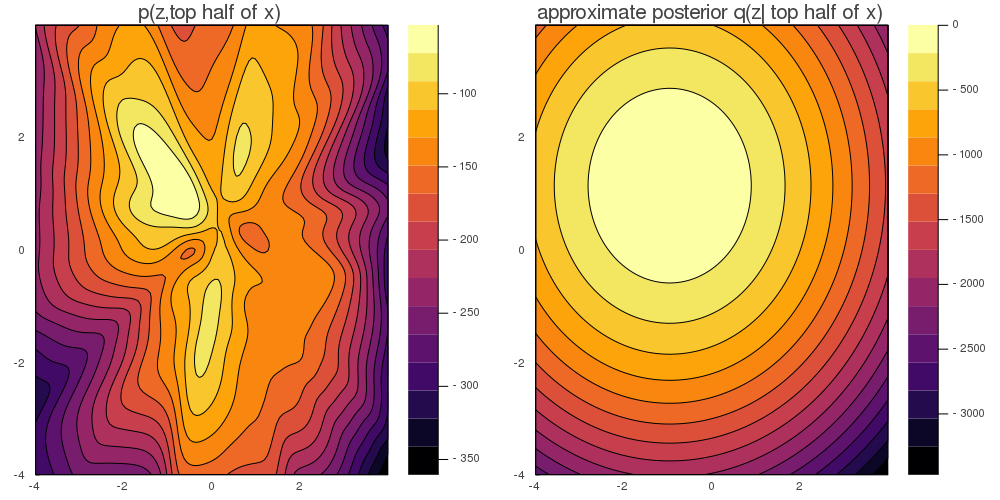
\includegraphics[width=15cm]{plots/4b_d.png}
  \caption{Contour Plots of Joint and Approximate Posterior on Top Half of a Sample}
\end{figure}

\begin{figure}[h]
  \centering
  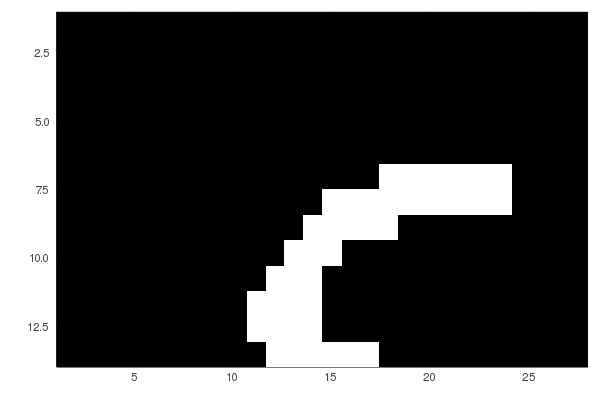
\includegraphics[width=5cm]{plots/4b_d_sample.png}
  \caption{Provided Sample (Top Half of a digit 5) to the Above Coutour Plots}
\end{figure}

\pagebreak

	\item {\bf [5 points]} True or false: Questions about the model and variational inference.
	
	There is no need to explain your work in this section.

\begin{enumerate}[label=(\alph*)]
	\item Does the distribution over $p(\text{bottom half of image $x$} | z)$ factorize over the pixels of the bottom half of image $x$? Yes. This is encoded in our model.
	\item Does the distribution over $p(\text{bottom half of image $x$} | \text{top half of image $x$})$ factorize over the pixels of the bottom half of image $x$? No. It may map to some distribution of intermediate z's before mapping back to image space which make it not factorized over the bottom half of given input x.
	\item When jointly optimizing the model parameters $\theta$ and variational parameters $\phi$, if the ELBO increases, has the KL divergence between the approximate posterior $q_\phi(z|x)$ and the true posterior $p_\theta(z|x)$ necessarily gotten smaller? No. It may be due to reconstuction term of the loss.
	\item If $p(x) = \mathcal{N}(x | \mu, \sigma^2)$, for some $x \in \mathbb{R}, \mu \in \mathbb{R}, \sigma \in \mathbb{R}^+$, can $p(x) < 0$? False
	\item If $p(x) = \mathcal{N}(x | \mu, \sigma^2)$, for some $x \in \mathbb{R}, \mu \in \mathbb{R}, \sigma \in \mathbb{R}^+$, can $p(x) > 1$? True
\end{enumerate}
  
\end{enumerate}

\section{Implementation Source Code}
See vae.jl for code.

\end{document}
